
\begin{frame}{Motivating Example}

Inferring population structure from genomic sequences.
\begin{itemize}
  \item[--] Genetic data from Taita thrush, an endangered bird species native to Kenya
  \citep{galbusera:2000:thrush}
  %{\color{blue} \href{https://web.stanford.edu/group/pritchardlab/publications/pdfs/Pritch%ardEtAl00.pdf}{(Pritchard et al. 2000)}}
  \item[--] Microsatellites sequences of 155 individuals at 7 loci.
\end{itemize}


\begin{figure}[!h]
\centering
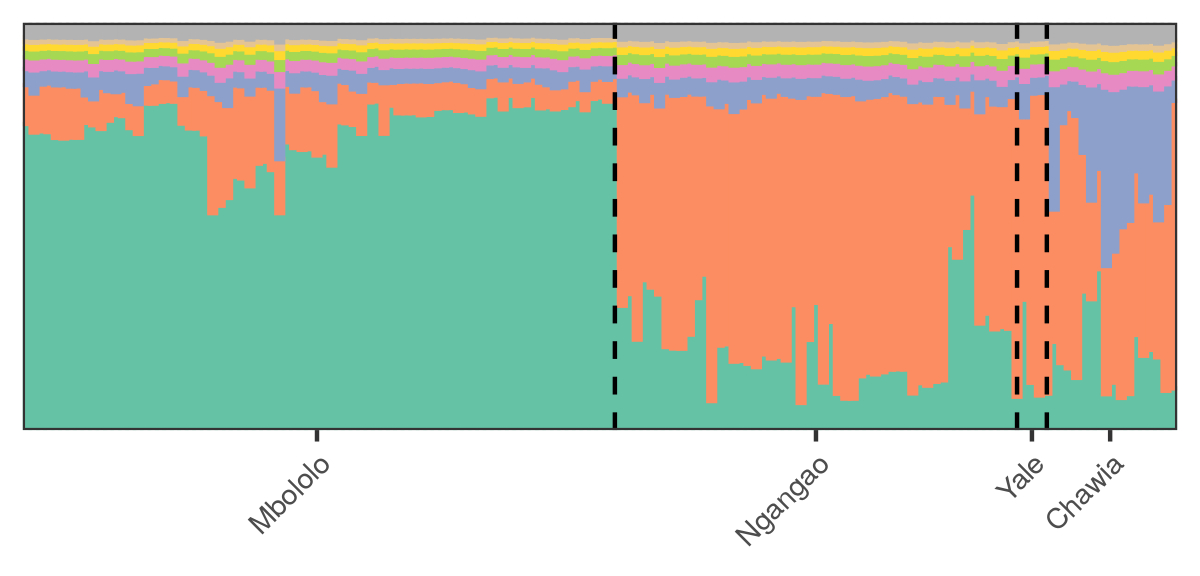
\includegraphics[width = 0.9\textwidth]{./figure/structure_init-1.png}
\end{figure}

\end{frame}

\begin{frame}{Motivating Example}

\begin{figure}[ht!]
\centering
\only<1-2>{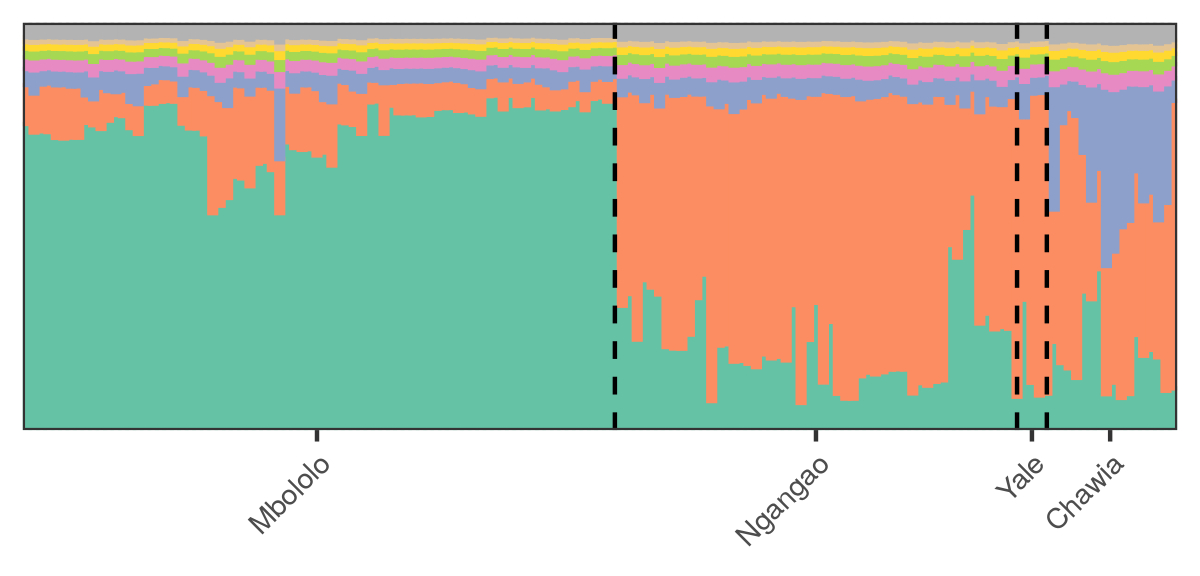
\includegraphics[width = 0.9\textwidth]{./figure/structure_init-1.png}}
\only<3>{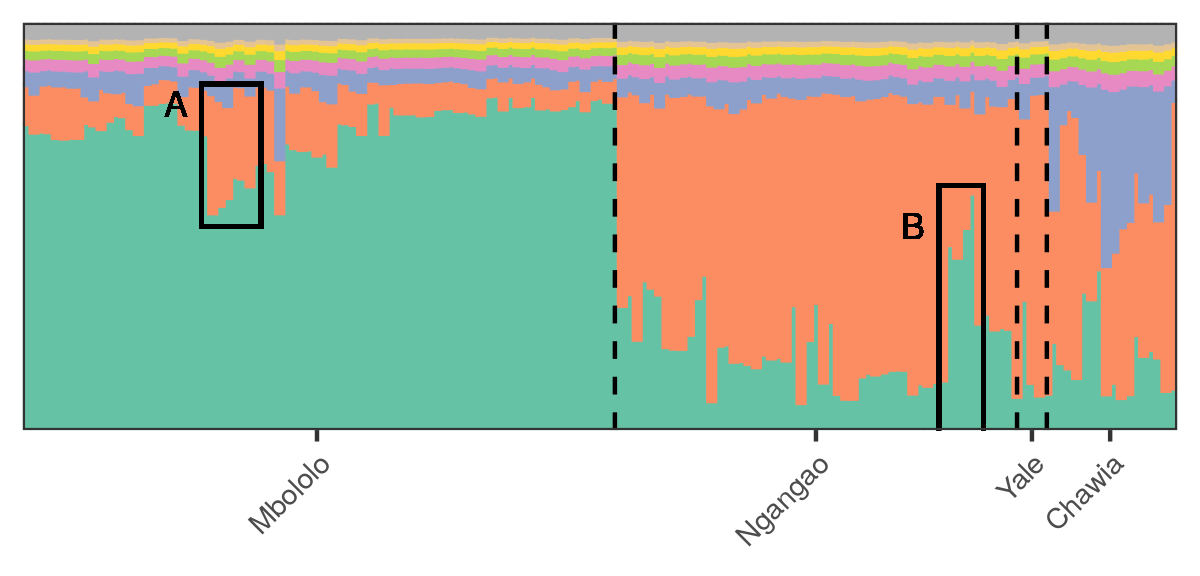
\includegraphics[width = 0.9\textwidth]{./figure/structure_migration-1.png}}
\end{figure}
\vspace{-1em}

%%%%%%%%%%%%%
% how many latent populations?
%%%%%%%%%%%%%
\only<1>{
%\textbf{How many latent populations (clusters) are present in the data set?}

- Three primary populations
{\large
\textcolor{pop1}{$\blacksquare$}
\textcolor{pop2}{$\blacksquare$}
\textcolor{pop3}{$\blacksquare$}
}.

- Many small, rare populations
{\large 
\textcolor{pop4}{$\blacksquare$}
\textcolor{pop5}{$\blacksquare$}
\textcolor{pop6}{$\blacksquare$}
\textcolor{pop7}{$\blacksquare$}
\textcolor{pop8}{$\blacksquare$}
}. 

{\bf Question: How many distinct populations (clusters) are there...}
\vspace{-0.5em}
\begin{itemize}
    \item ...in this dataset?
    \item ...with more than $N$ loci?
    \item ...in a future dataset of the same size?
\end{itemize}
\vspace{3.5em}
}



%%%%%%%%%%%%%
% coclustering
%%%%%%%%%%%%%
\only<2-3>{
Individuals are generally clustered by geographic locations:
\begin{minipage}{0.3\textwidth}
 Mbololo $\approx$ {\large \textcolor{pop1}{$\blacksquare$}}
\end{minipage}
\begin{minipage}{0.3\textwidth}
 Ngangao $\approx$ {\large \textcolor{pop2}{$\blacksquare$}}
\end{minipage}
\begin{minipage}{0.35\textwidth}
Chawia $\approx$
    {\large 
    \textcolor{pop1}{$\blacksquare$} + 
    \textcolor{pop2}{$\blacksquare$} + 
    \textcolor{pop3}{$\blacksquare$}}
\end{minipage}

\textbf{Question: Which individuals cluster together?}

Exceptions to the clustering give evidence of historical migrations.
}

\only<2> {
% so that the figure aligns across the \only ....
% is there a better way to do this?
\vspace{2em}
}
\only<3>{
For example, the groups of individuals in A and B suggest migration
between the Mbololo and Ngangao locations. 
}
\end{frame}



\begin{frame}{Motivating Example}
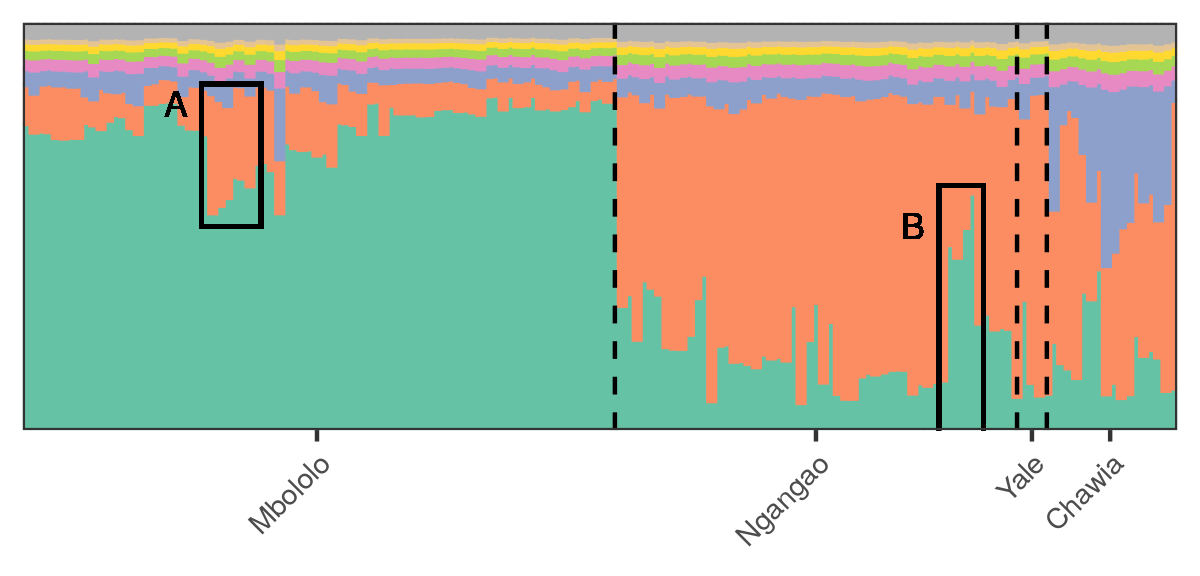
\includegraphics[width = 0.9\textwidth]{./figure/structure_migration-1.png}

How many distinct clusters are there?
%
Which individuals cluster together?

A \textbf{discrete Bayesian nonparametric (BNP)} model makes these questions 
amenable to Bayesian inference...

...but the answer may depend on the \textbf{prior you choose.}

\end{frame}


\begin{frame}{Motivating Example}

\begin{figure}[!h]
\centering
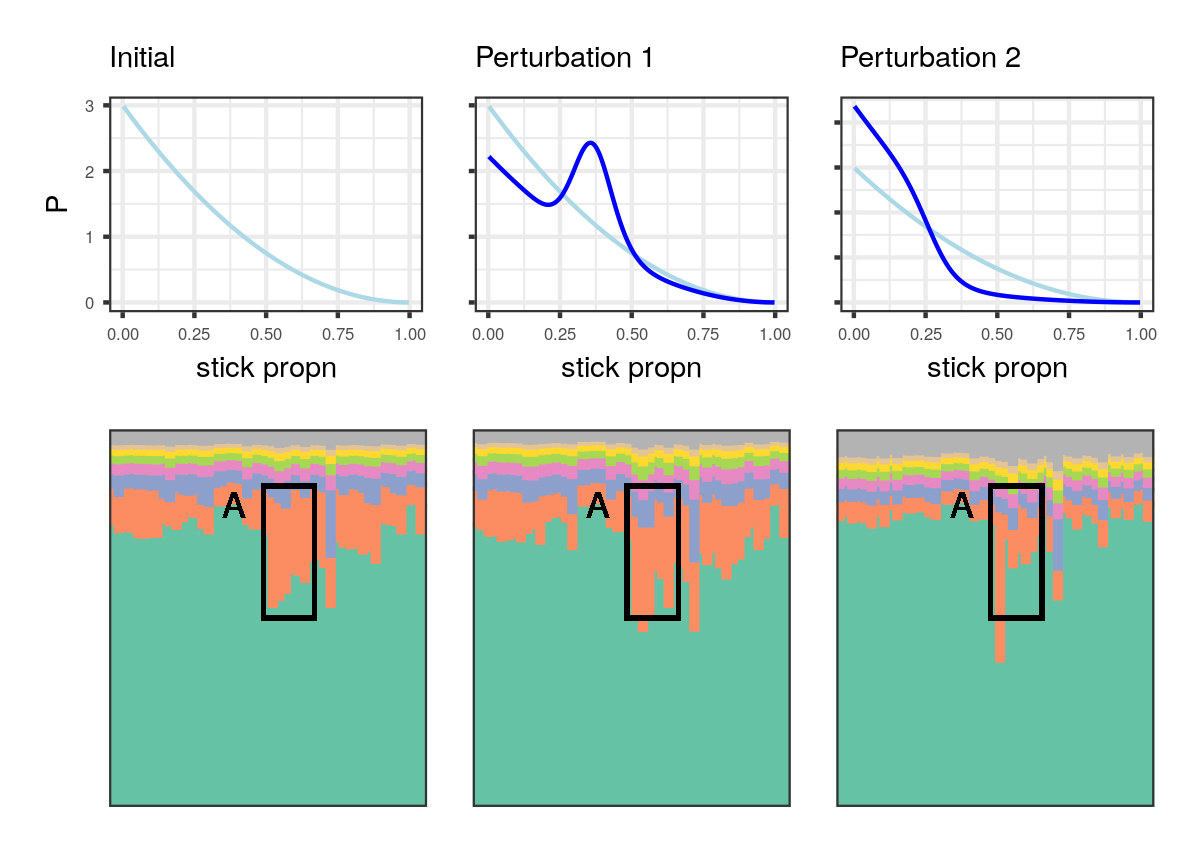
\includegraphics[width = \textwidth]{./figure/mbololo_motivating_ex-1.png}
\end{figure}

\end{frame}



\begin{frame}{Research Problem}

A discrete Bayesian nonparametric (BNP) model makes scientific
questions amenable to Bayesian inference.

\pause

We approximate the exact posterior using variational Bayes (VB).

\pause

\textbf{Question}: How sensitive is the VB approximation, and the resulting
inferences, to BNP model choices?

\pause

\textbf{Problem}: Re-running VB for multiple model choices is expensive.

\pause

\textbf{We propose}: A linear approximation to efficiently
estimate BNP sensitivity from a single run of VB.  The linear approximation
can both:
\begin{itemize}
    \item Provide approximate sensitivity with no refitting, or
    \item Guide the choice of priors for refitting.
\end{itemize}

\end{frame}



\begin{frame}{Outline}
\begin{itemize}
\item The BNP model
\vspace{0.1in}

\item The variational approximation
\vspace{0.1in}

\item Hyperparameter sensitivity
\vspace{0.1in}

\item Functional sensitivity and influence functions
\vspace{0.1in}

\item Results on population genetics modeling of the Taita thrush
\vspace{0.1in}

\end{itemize}
\end{frame}
